\section{背景及び目的}

\subsection{背景}

\subsubsection{ゲームを超えたXRへの期待の高まり}

昨今VR(Virtual Reality)やAR(Augmented Reality)などのXRのブームが再来している.
IDCの2022年3月のレポート~\cite{idc}によると,世界のAR/VRヘッドセットの市場は2021年で92.1\%
成長し,1000万台を超えるヘッドセットが出荷された.
また,ヘッドセットの市場は2026年までに年平均35.1\%で成長し,2026年に出荷されるヘッドセットは
5000万台を超えると予想されている(図\ref{fig:idc}).

\begin{figure}[htbp]
  \begin{minipage}[b]{0.50\linewidth}
    \centering
    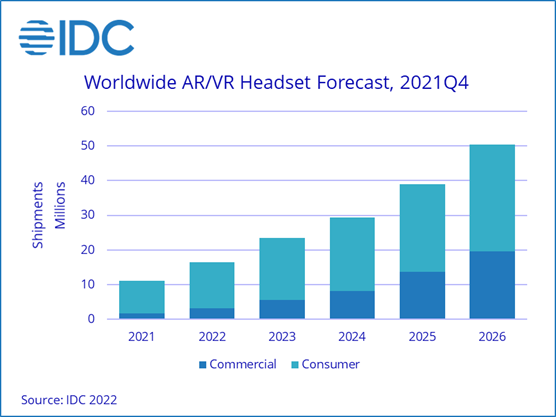
\includegraphics[keepaspectratio, width=0.9\linewidth]{fig/idc.png}
    \caption{IDCによる世界のAR/VRヘッドセットの市場予測}
    \label{fig:idc}
  \end{minipage}
  % \begin{minipage}[b]{0.50\linewidth}
  %   \centering
  %   \includegraphics[keepaspectratio, width=0.9\linewidth]{fig/workrooms.jpeg}
  %   \caption{Horizon Workrooms (Meta社)}
  %   \label{fig:workrooms}
  % \end{minipage}
  \begin{minipage}[t]{0.50\linewidth}
    \centering
    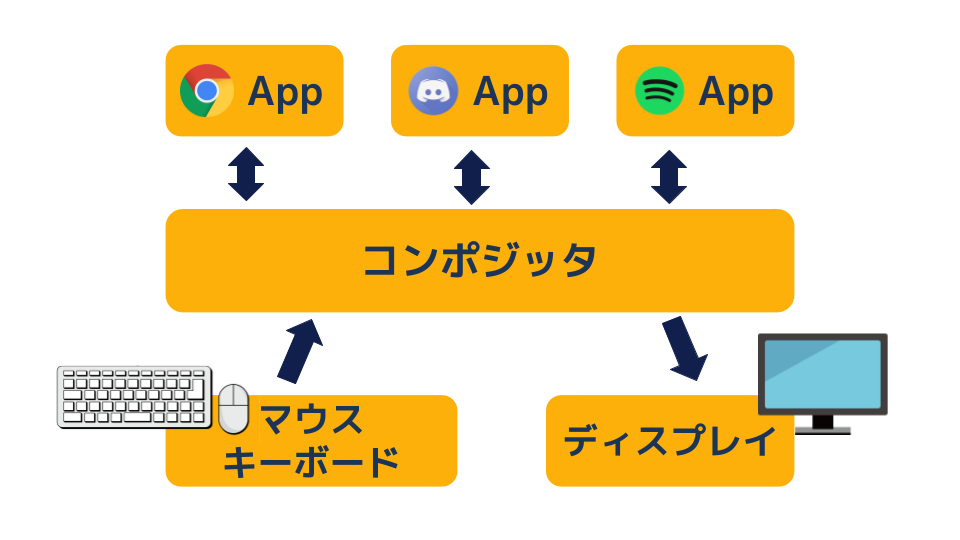
\includegraphics[keepaspectratio, width=\linewidth]{fig/2d-windowing-system.png}
    \caption{2D Windowing Systemの概要図}
    \label{fig:2d-windowing-system}
  \end{minipage}
\end{figure}


XRの利用シーンは,コンシューマ向けのVR/ARマーケットではゲームなどのエンターテイメント向けの利用が目立つが,
VRChat\footnote{VRChant Inc. ``VRChat'' \url{https://hello.vrchat.com/} (accessed on 24 Jan, 2023)}
やHorizon World\footnote{Facebook Technologies, LLC. ``Horizon Worlds'' \url{https://www.oculus.com/horizon-worlds/} (accessed on 24 Jan, 2023)}
といったコミュニティに重きを置いた利用も活発になり,コンピュータネットワーク上の
新たな世界を指すメタバースという言葉が流行っている.
また,職業支援や職業訓練への応用も進んでおり,
医療\cite{Gallagher2005-gv}や航空宇宙\cite{aerospace},軍事\cite{military},
農業\cite{agriculture}などさまざまな分野での研究が活発で,
実際に産業界での導入も進んでいることがIDCのレポート\cite{idc-2022}からわかる.

このようなVR/ARを用いたアプリケーションがゲームや特定のシーンだけの利用にとどまらず,
多様化していることがわかる.

\subsubsection{通常の2Dデスクトップ環境におけるWindowing Systemについて}

今日において GUI デスクトップ環境ではWindowing System
(Linuxでは X11やWayland,macOSではQuartz compositorなど)が用いられており,
これによって優れた作業環境を提供できている.
Windowing Systemではアプリケーションが直接自身の描画内容をディスプレイに出力したり,
マウスなどのインプットデバイスからの入力を受け取ったりせず,ディスプレイサーバや
コンポジッタと呼ばれるソフトウェアとのやりとり(プロセス間通信)を介して
これらのハードウェアを扱うようにしている(図\ref{fig:2d-windowing-system}).
コンポジッタの主な役割は,
\begin{itemize}
  \item 複数のアプリケーションから描画内容を受け取り,
        それらを一枚のスクリーンに合成してディスプレイに表示する.
  \item マウスやキーボードなどのハードウェアからの入力を適切なアプリケーション
        (ユーザがフォーカスしているアプリケーションなど)に割り振る.
  \item ドラッグ\&ドロップなどのアプリケーション間のデータ共有の仕組みを提供する.
\end{itemize}
などである.これによって,開発元の異なる複数のアプリケーションを同じディスプレイ上にウィンドウが
自然に重なる形で表示したり,また1つのマウスやキーボードでフォーカスを切り替えながら複数の
アプリケーションを操作したりでき,マルチアプリケーション・マルチタスクの環境が実現されている.

\begin{figure}[htbp]
  \begin{minipage}[t]{0.50\linewidth}
    \centering
    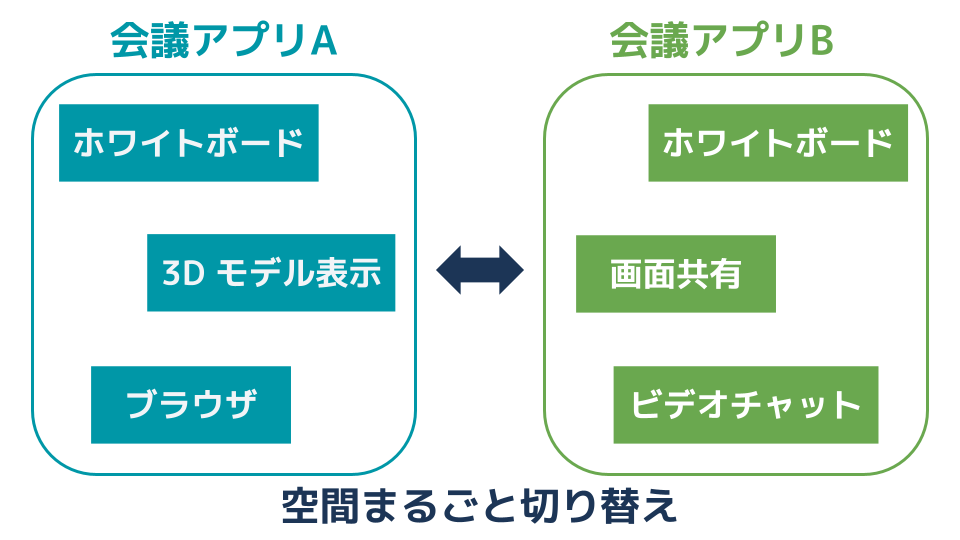
\includegraphics[keepaspectratio, width=0.9\linewidth]{fig/xr-app-switch.png}
    \caption{
      現状のXRアプリケーションの切り替え.アプリケーションの切り替えは,空間内の全ての
      機能を切り替えることになってしまう.
    }
    \label{fig:xr-app-switch}
  \end{minipage}
  \begin{minipage}[t]{0.50\linewidth}
    \centering
    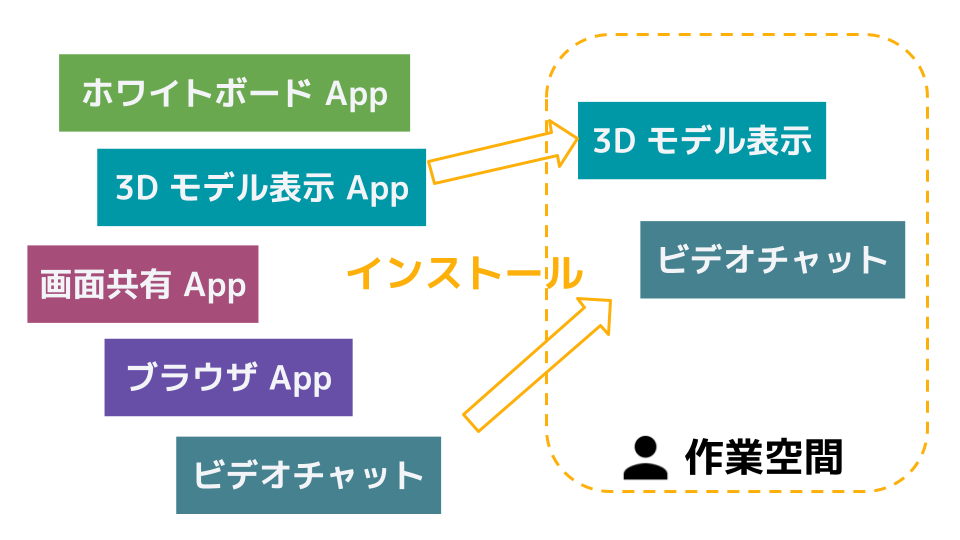
\includegraphics[keepaspectratio, width=\linewidth]{fig/xr-app-install.png}
    \caption{XR空間でユーザが好きなアプリケーションをインストールして同時に複数使う.}
    \label{fig:xr-app-install}
  \end{minipage}
\end{figure}

\subsubsection{現状のXRアプリケーションについて}

2Dのデスクトップ環境では複数のアプリケーションが同時に使用・連携できるのに対し,
現状のXRアプリケーションは基本的に1つのメインアプリケーションがユーザの視界の全てを支配する.
そのため,アプリケーションを切り替えると,空間ごと切り替えることに
なってしまい(図 \ref{fig:xr-app-switch}),XRアプリケーションは,その空間に必要な
機能をその1つのアプリケーションが全て実装している必要がある.
1つのアプリケーションが1つの世界観を作り出すXRゲームなどにおいてはこれで問題ないが,
作業空間や日常生活のアシスタントとしてXRを用いたい場合は問題が生じる.
作業や日常生活に必要な機能は個人ごとに大きく異なり多様性が大きいため,1つのアプリケーションが
全てのニーズに応えて機能を実装するのは現実的に不可能である.
例えば図\ref{fig:xr-app-switch}の例で,会議アプリAを利用しているユーザが会議アプリBの
画面共有のような機能を3Dモデルの表示と一緒に使いたいと思っても,
会議アプリAの開発元が画面共有機能を追加しない限りそれは不可能である.

% 一部のXR空間では簡易的に複数のアプリケーションを重ねて表示する機能を提供する仕組みも存在するが,
% それについては\ref{section:openxr-overlay}で詳しく言及する.
% また特に,このような汎用的な会議アプリケーションに対して,ニーズの割合が小さい,例えば
% 医療CTスキャンの結果を表示するようなアプリケーションは実装されないだろう.
% そして逆に医療CTスキャンの結果を表示したいモチベーションの開発者が同時に会議アプリケーション
% としての機能を実装することもないと考えられるため,XR会議をしながらCTスキャンの結果を
% 見るという世界が実現する可能性は低い.

\subsubsection{何が必要か}

特に作業空間や日常生活のサポートとしてのXRでは,全ての機能を1つのアプリケーションが実装するのではなく,
図\ref{fig:xr-app-install}のように個々の機能がそれぞれアプリケーションとして
異なる開発元によって開発され,ユーザが必要な機能のアプリケーションをインストールすることで
自分に最適な作業空間を作れるようにするべきである.
% textlint-disable
このようにお気に入りのアプリケーションをインストールし,複数のアプリケーションを同時に
% textlint-enable
利用することで作業空間を作り上げていくことは,2Dのデスクトップ環境では当然のように
行われていることだが,XRの作業空間では達成できていない.
XRにもこのようなマルチアプリケーション・マルチタスクの作業環境が求められる.

\subsection{未踏アドバンスト事業実施以前の状況}
\label{section:current-status}

XRでのマルチアプリケーション・マルチタスクの作業環境を実現するためには,
複数のアプリケーションの描画情報を1つの空間に合成して表示したり,
入力デバイスからの入力を適切なアプリケーションに割り振ったりする,
2D デスクトップ環境でのWindowing Systemが担当している機能が必要となる.
そこで本プロジェクトでは未踏IT人材発掘・育成事業の支援を受けてXR向けのWindowing System,
"ZIGEN"を開発してきた.

ZIGENではWindowing SystemのライブラリであるWaylandの上で,XR用にディスプレイサーバと
アプリケーション間のプロトコルを定義し,参照実装としてのディスプレイサーバ, "ZEN" を実装した.
また既存の2Dアプリケーション(Google Chromeなど)を表示するためのアプリケーションである
"zmonitors"やその他サンプルの3Dアプリケーションを実装した.
これによって主な特徴として以下のことができるようになっている.

\begin{enumerate}
  \item \textbf{空間の一部を占めるような複数のアプリケーションをそれぞれ起動し,
          同時に表示する(図\ref{fig:multi-app}).}\\
        それぞれのアプリケーションはターミナルなどからプロセスとして立ち上げ,
        % textlint-disable
        OpenGLに似たAPIのZIGENプロトコルに従って頂点バッファ・頂点配列・テクスチャ・
        シェーダ(GLSL)・その他オプションをディスプレイサーバに伝えることで描画を行う.
        % textlint-enable
        ディスプレイサーバ側では受け取った描画情報を各アプリケーションどうしの
        前後関係などが正しく考慮された形で合成し,1つの空間に描画している.
        各アプリケーションはOpenGLで直接描画する場合とほとんど同じインターフェースで
        描画できるため,描画の自由度は大きく損なわない.また他のアプリケーションのことを
        知らずに描画が行え,開発元の違うアプリケーションどうしでも自然に重ね合わされる.
  \item \textbf{Rayとキーボードを用いて適切に入力をアプリケーションに伝えられる
          (図\ref{fig:ray-input}).}\\
        ZIGENではRay(半直線)とキーボードを用いてアプリケーションを操作する.
        Rayは2Dデスクトップのポインタに相当し,アプリケーションへのクリックやスクロール,
        ドラッグといった操作を与える.さらに,Rayによってアプリケーションへ
        フォーカスでき,キーボードイベントはフォーカスしたアプリケーションへのみ渡される.
  \item \textbf{既存の2Dアプリケーションを利用できる(図\ref{fig:2d-apps}).}\\
        Google Chromeなどの既存の2Dアプリケーションが修正なしでそのまま動作し,
        Rayを用いて操作できる(Rayと2Dウィンドウとの交点がカーソルとして機能する).
        この機能を提供するために作成した"zmonitors"というソフトウェアは画面共有のような
        仕組みを用いるのではなく,図\ref{fig:zmonitors}のように2Dのディスプレイサーバとして
        Google Chromeなどと2D Windowing System(Wayland)のプロトコルでやりとりを
        行いつつ,かつ3DアプリケーションとしてZIGENディスプレイサーバ(ZEN)とやりとりを行い,
        3D空間上に2Dアプリケーションを表示している.画面共有やVNCなどではなく,
        ディスプレイサーバから実装することによって,画面更新をより効率的に行えたり,
        HMD(ヘッドマウンテッドディスプレイ)と2Dアプリケーションが完全にフレーム同期を
        行えたりする利点がある.これを実現するためにZIGENのプロトコルは既存の
        2D Windowing Systemと変換可能に設計されている.
  \item \textbf{2Dと3Dの垣根を越えたドラッグ \& ドロップ(図\ref{fig:dnd}).}\\
        ZIGENでは既存の2Dアプリケーションと3Dアプリケーションとの間でドラッグ \& ドロップが
        可能である.このようなことが可能であるのもZIGENが2DのWindowing Systemと
        変換可能に設計され,zmonitorsを2Dディスプレイサーバの部分から実装している利点であり,
        このような2Dと3D アプリケーション間のドラッグ \& ドロップを実装したのは
        調べる限り世界で初である.
\end{enumerate}

現状の開発成果物に関しては動画のデモがあるので,ドラッグ \& ドロップの様子や,クオリティなどに
関してはぜひそちらを参照されたい.
\begin{itemize}
  \item \textbf{デモ動画:\url{https://sites.google.com/view/zigen/demo}}
\end{itemize}

\begin{figure}[htbp]
  \begin{minipage}[t]{0.50\linewidth}
    \centering
    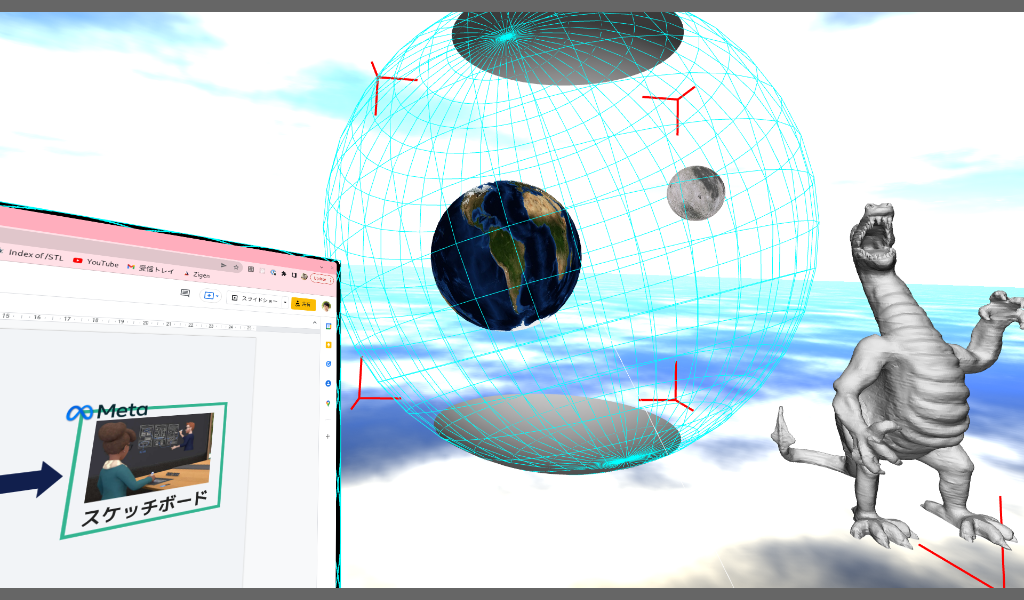
\includegraphics[keepaspectratio, width=\linewidth]{fig/multi-app.png}
    \caption{
      複数3Dアプリケーションの表示.左は既存の2Dアプリケーション(Google Chrome)
      中心はサンプルで作成した天体を表示・編集するアプリケーション,
      右は3Dファイルを表示するアプリケーション.また背景の空も1つのアプリケーションであり,
      ユーザが任意に変更可能である.
    }
    \label{fig:multi-app}
  \end{minipage}
  \begin{minipage}[t]{0.50\linewidth}
    \centering
    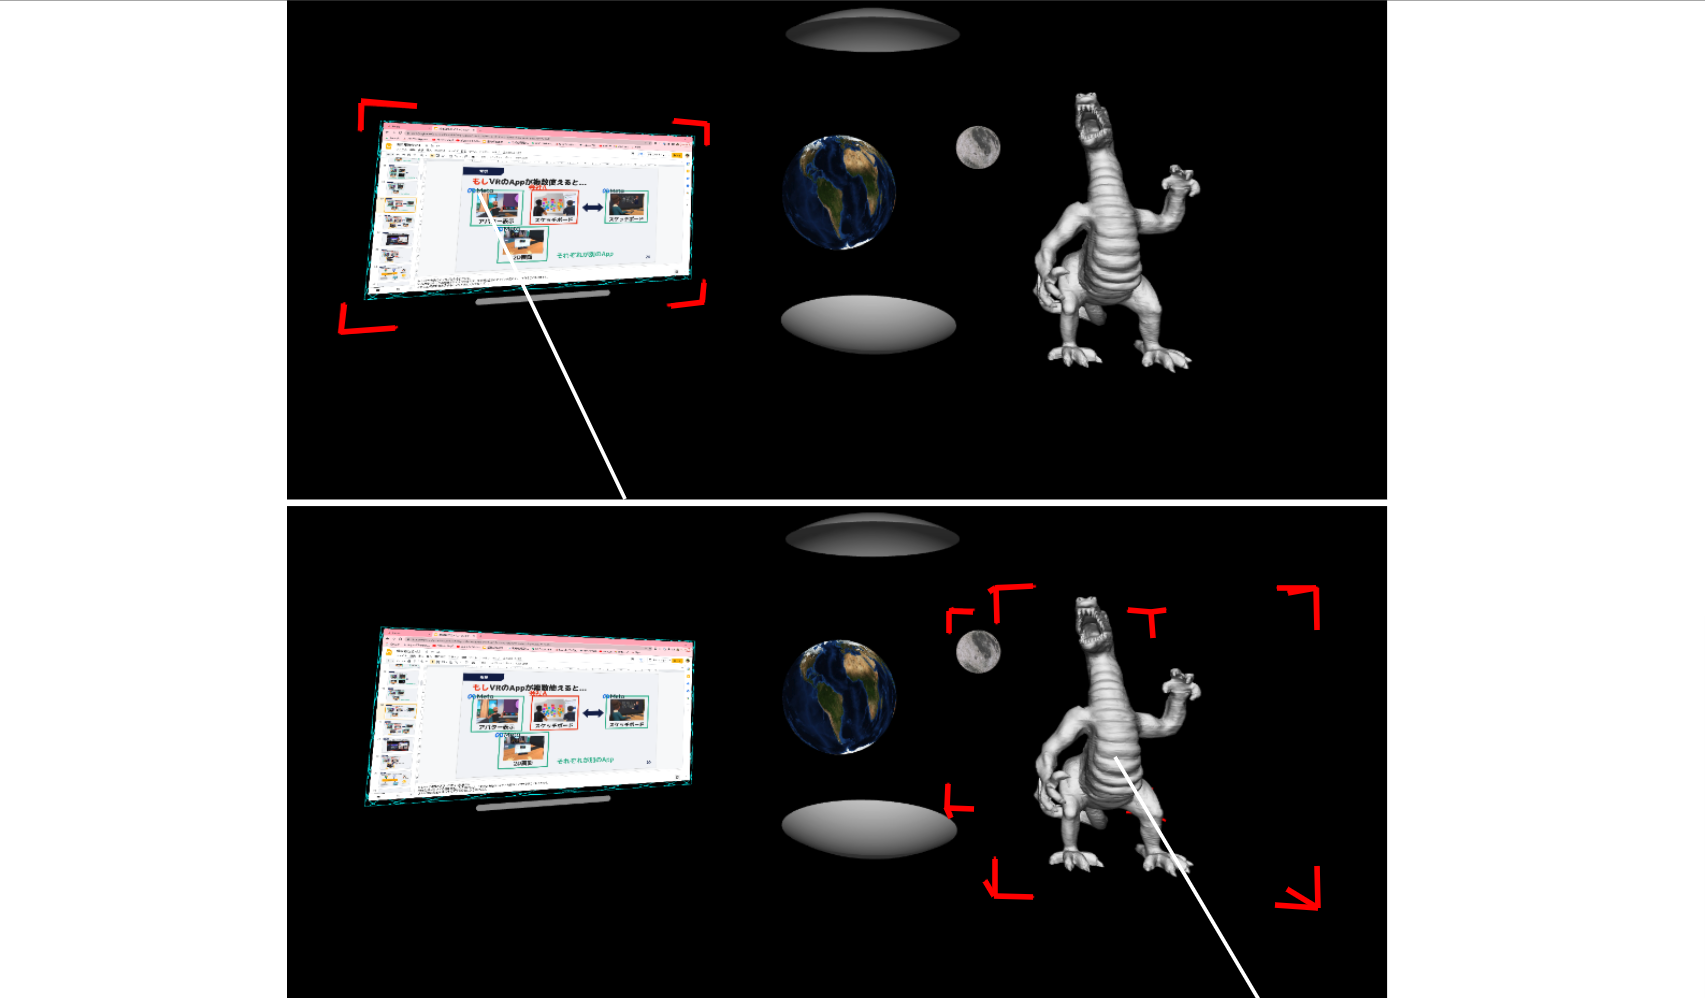
\includegraphics[keepaspectratio, width=\linewidth]{fig/ray-input.png}
    \caption{
      Rayによって3Dアプリケーションへのフォーカスを切り替えている様子.
      上段は一番左のアプリケーションに,下段は一番右のアプリケーションにフォーカスしており,
      アプリケーションがハイライトされている様子がわかる.
    }
    \label{fig:ray-input}
  \end{minipage}
\end{figure}

\begin{figure}[htbp]
  \begin{minipage}[t]{0.50\linewidth}
    \centering
    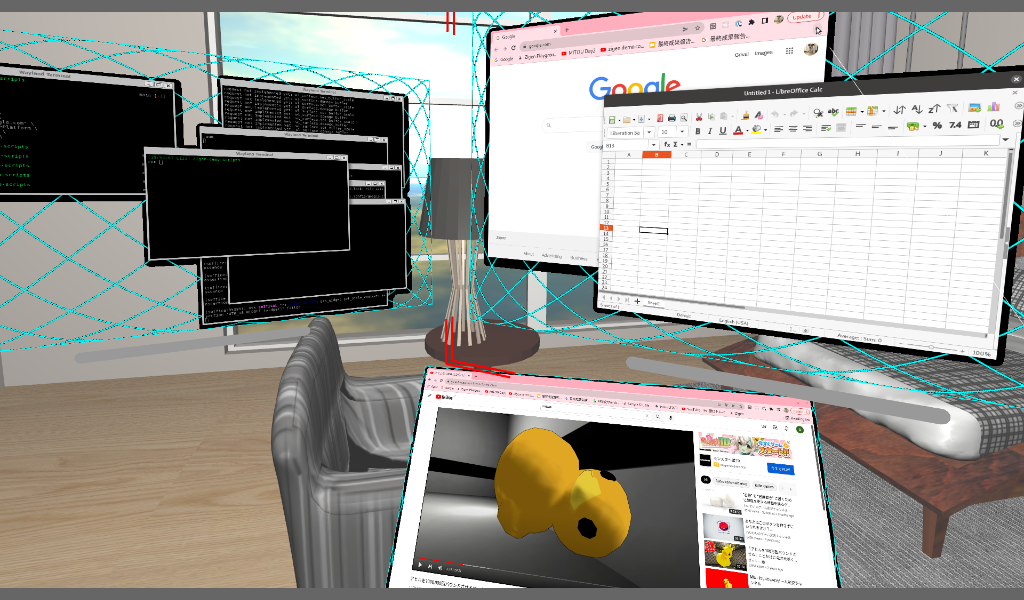
\includegraphics[keepaspectratio, width=\linewidth]{fig/2d-apps.png}
    \caption{
      ブラウザなどの既存の2Dアプリケーションが修正なしでそのまま動作する.
    }
    \label{fig:2d-apps}
  \end{minipage}
  \begin{minipage}[t]{0.50\linewidth}
    \centering
    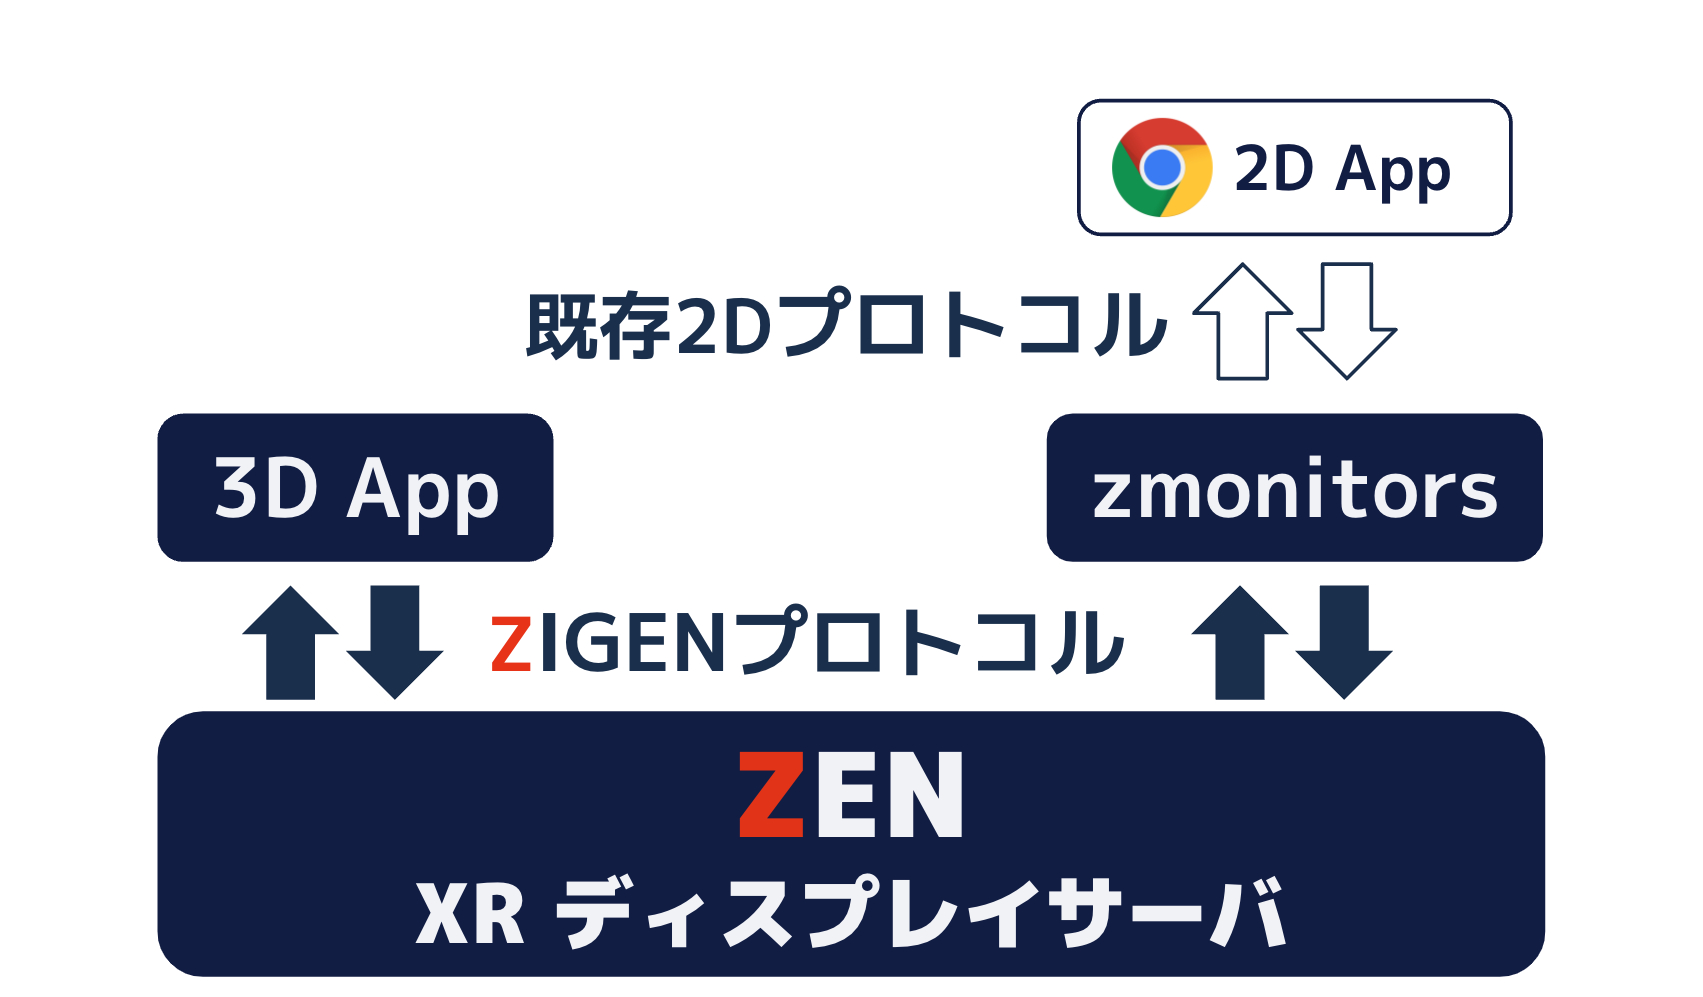
\includegraphics[keepaspectratio, width=\linewidth]{fig/zmonitors.png}
    \caption{
      既存の2Dアプリケーションを3Dアプリケーションに変換するzmonitors.
    }
    \label{fig:zmonitors}
  \end{minipage}
\end{figure}

\begin{figure}[htbp]
  \centering
  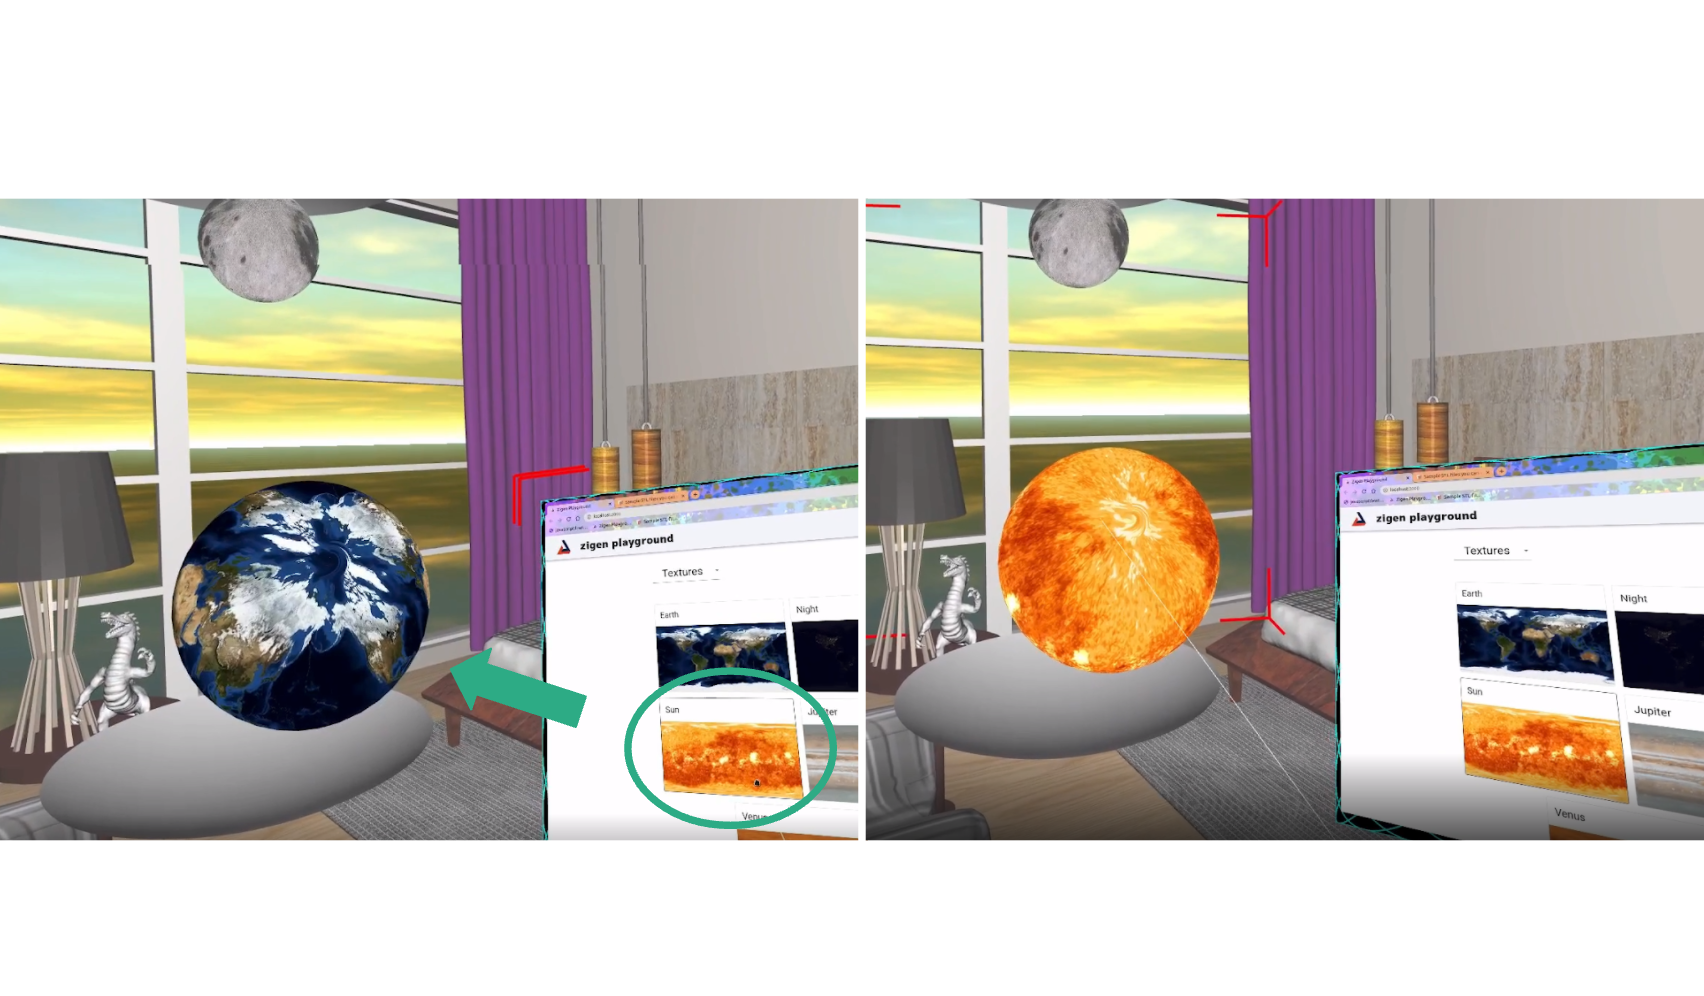
\includegraphics[keepaspectratio, width=0.7\linewidth]{fig/dnd.png}
  \caption{
    Google Chromeから天体を表示・編集する3Dアプリケーションに,天体のテクスチャを
    ドラッグ \& ドロップすることで,天体を地球から太陽に変更する様子.
  }
  \label{fig:dnd}
\end{figure}

\subsection{目的}
\label{section:objective}

本プロジェクトの目的はXR空間にWindowing Systemを導入することで
XR空間にマルチアプリケーション・マルチタスクの環境を提供することである.
\ref{section:current-status}で述べたように,本プロジェクトは未踏IT人材発掘・育成事業
% textlint-disable
において,メインのコンセプトについて概念実証を行ってきが,これをさらに社会へ実装するため,
% textlint-enable
未踏アドバンストでは以下のより詳細な目的を設定した.

\begin{enumerate}
  \item \textbf{実用レベルのXRデスクトップ環境を提供する.}\\
        ユーザが日常で使うデスクトップ環境を
        提供するためには,単純にディスプレイサーバを実装するだけでは足りず,
        アプリケーションラウンチャーなどのグラフィカルシェルと呼ばれる部分の実装などが必要になる.
  \item \textbf{ユーザと3Dアプリケーション開発者からなるエコシステムを形成する.}\\ %TODO: ここは伝わる言い方になってない。改善する。
        本プロジェクトが目指す世界の特徴として,XR空間全体ではなく各機能がそれぞれ
        アプリケーションとなることで,機能ごとに市場競争が生じ,
        また開発者も特定の機能だけをうまく実装すればよいことになる.
        これによって現在より多様な機能や多様な開発者が生まれ,作業空間としてのXRは
        より洗練された空間になる.この世界の実現のため,まずは個人の開発者が空間の改善を行え,
        それをユーザに使ってもらえる仕組みを提供していく.
  \item \textbf{多くのユーザに実際に試してもらう.}\\
        未踏IT人材発掘・育成事業では実際にユーザに使ってもらい,生のフィードバックを
        多くもらうまでは至らなかった.これを達成するためにはイベントの参加・開催,
        多様なハードウェアへの対応,認知度向上などに関してするべきことがある.
  \item \textbf{XR世界を作り上げているコミュニティでのプレゼンスを高める.}\\
        XRの環境は今もまだまだ開発段階であり,多くの開発者がXR空間の改善のために活動している.
        その中でプロジェクトの価値を認められることはOSSとしての継続的な開発と技術の浸透の
        ために重要である.また,XRの環境は多くの技術を組み合わせた世界であり,本プロジェクトが
        長期的なスパンで成功するためには,他のOSSプロジェクトなどの協力が不可欠であり,
        その点でも重要となってくる.(例えばパフォーマンス向上のためにはOpenGLにおいて
        Extensionの開発などが求められる.)また,本プロジェクトは技術上の制約で
        Linux上でしか動作しないが,他のOSに対しても影響を与え,XR Windowing Systemの
        コンセプトを広く普及させることにも繋がる.
\end{enumerate}
